\documentclass{article}

\usepackage{enumerate}
\usepackage{amssymb}
\usepackage{amsmath}
\usepackage{algorithm}
\usepackage{physics}
\usepackage{listings}
\usepackage[noend]{algpseudocode}
\usepackage{graphicx}

\graphicspath{ {./} }

\topmargin=-0.45in
\evensidemargin=0in
\oddsidemargin=0in
\textwidth=6.5in
\textheight=9.0in
\headsep=0.25in

\title{Chem 195: Problem Set 12}
\author{Michael Stephen Chen}


\begin{document}
\maketitle
\pagebreak

\section*{Problem 1}
\begin{enumerate}[i.]
  \item Let's first compute the force along the direction $x$. To do that we note that,
    $$F_x = -\frac{\partial u}{\partial x} = -\frac{\partial u}{\partial r}\frac{\partial r}{\partial x}$$

    To calculate $u'(r) = \frac{\partial u}{\partial r}$,
    \begin{align}
      u(r) &= 4(r^{-12} - r^{-6}) - 4(r_{cut}^{-12}-r_{cut}^{-6}) \\
      u'(r) &= \frac{\partial}{\partial r} 4(r^{-12} - r^{-6}) - 4(r_{cut}^{-12}-r_{cut}^{-6}) \\
      &= -48r^{-13} + 24r^{-7} \\
      &= -48 \left[ r^{-13} - \frac{1}{2}r^{-7} \right] \\
    \end{align}

    To calculate $\frac{\partial r}{\partial x}$
    \begin{align}
      \frac{\partial r}{\partial x} &= \frac{\partial}{\partial x} (x^2 + y^2)^{1/2} \\
      &= \frac{x}{(x^2 + y^2)^{1/2}} \\
      &= \frac{x}{r} \\
    \end{align}

    Putting this all together we get,
    \begin{align}
      F_x &= -\frac{\partial u}{\partial r}\frac{\partial r}{\partial x}\\
      &= 48 \left[ r^{-14} - \frac{1}{2}r^{-8} \right] x \\
    \end{align}

    The result is analogous for $F_y$, thus
    $$\vec{F} = 48 \left[ r^{-14} - \frac{1}{2}r^{-8} \right] \vec{r}$$

    where $\vec{r} = \left[ x, y \right]^T$.

  \item The force on a particle in the lattice configuration is essentially $\left[0, 0 \right]$, however due to numerical errors the actual computed force components along the x and y directions is on the order of $10^{-14}$. All particles in this configuration are identical given that we are using periodic boundary conditions so they should all have the same force components.

  \item The force on the shifted particle is now $\left[ 0.961, 0\right]$ while the force on the neighbor that is above it in the y-direction is $\left[ 0.118, 0.025\right]$. Yes it does matter because force is a vector that is dependent on the distance vector between the particles (which is different amongst the neighboring particles in relation to the shifted one).
\end{enumerate}


\section*{Problem 2}
\begin{enumerate}[i.]
  \item See \textit{LJSimulation.m}

  \item A plot of the potential, kinetic, and total energies over the course of the simulation is shown below
    \begin{center}
      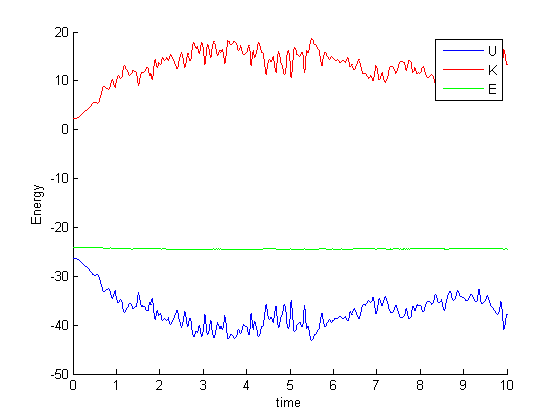
\includegraphics[scale=0.5]{2ii}
    \end{center}

  \item We can get a feel for the magnitude of the average velocities by observing the average kinetic energies in the plot above (with kinetic energy being proportional to the squared norm of the velocity). We see that the average velocity seems to drift (increasing in this case) until it reaches some sort of equilibrium and then the magnitude of the velocity seems to fluctuate randomly about that equilibrium value.

  \item The relationship between kinetic energy and temperature is as follows for our simulation where $d=2$ (in reduced units),
    $$\langle K \rangle = \frac{d}{2}NT = NT$$

    Therefore,
    \begin{align*}
      \langle T_{eff} \rangle &= \langle \frac{2K}{d(N-1)} \rangle \\
      &= \frac{\langle K \rangle}{(N-1)} \\
      &= \frac{N}{(N-1)} T\\
      &\approx T
    \end{align*}

    I'm asssuming the $N-1$ as opposed to $N$ is to correct for some sample bias, analogous to the formula for the sample variance?

  \item A plot of $T_{eff}$ over the course of the simulation is shown below
    \begin{center}
      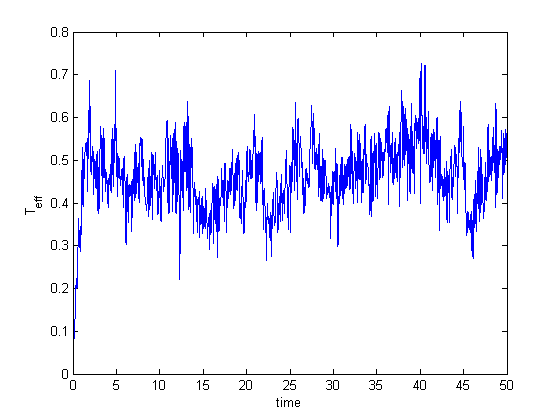
\includegraphics[scale=0.5]{2v}
    \end{center}

  \item The average effective temperature over the course of the simulation for one of the runs was $T_{eff}=0.4669$. However this average fluctuates considerably (I've seen some around 0.32 and other times around 0.51). 

    I would expect a closer correspondance for a larger system (where $N$ is larger). This is because the calcualated mean for $K$ should converge to the true mean as $N\rightarrow \infty$ (Central Limit Theorem); $K$ is part of our equation for determining $T_{eff}$. We also see in part (iv), $\langle T_{eff} \rangle = \frac{N}{(N-1)} T$ and $\frac{N}{N-1}$ will approach 1 as $N\rightarrow \infty$. 
\end{enumerate}


\section*{Problem 3}
\begin{enumerate}[i.]
  \item Below is a plot of $g(r)$ vs $r$ for $\rho=0.75$ and $T=0.45$.
    \begin{center}
      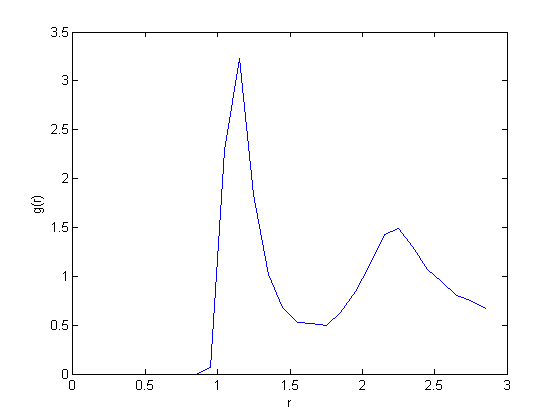
\includegraphics[scale=0.5]{3i}
    \end{center}

    Qualitatively the results appear to be similar to our MC sampling results; both plots have the same characteristic peak at roughly the same radii values.

  \item Below is plot of the radial distribution function for various densities
    \begin{center}
      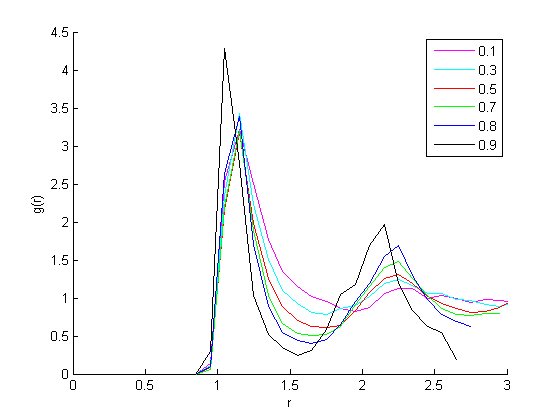
\includegraphics[scale=0.7]{3ii}
    \end{center}

  \item Below is plot of the radial distribution function for various densities
    \begin{center}
      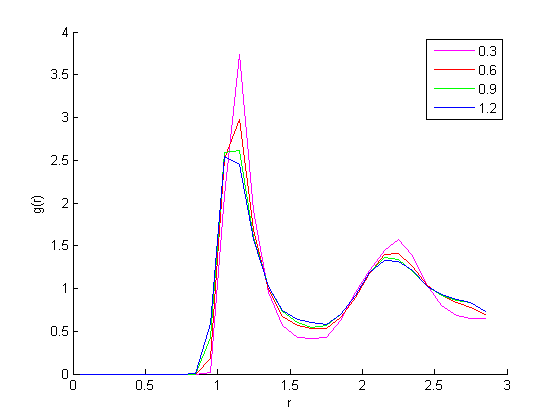
\includegraphics[scale=0.7]{3iii}
    \end{center}

  \item From examining the plot above, we see that both the peaks and the ``divots'' of the radial distribution function become less pronounced with increasing temperature. Physically the radial distribution function $g(r)$ is reflective of, as the name implies, the distribution of other particles at distances $r$ from a tagged particle. So a peak at $r$ means that there is a relatively high probability of finding another particle at $r$ while a ``divot'' implies that it is relaively uncommon too find a particle at $r$. So it makes sense that the peaks become less pronounced with increasing temperature, because the particles have higher average velocities and thus tend to sample more of the space (so counteracting the locality-inducing effects of the interparticle potentials). Put another way, the particles move around more at higher temperatures.
\end{enumerate}

\section*{Problem 4}
\begin{enumerate}[i.]
  \item We first note that
    $$C(0) = \langle v(0) \cdot v(0) \rangle = \langle |v(0)|^2 \rangle = \langle v^2 \rangle$$
    Then plugging that into the equation relating the average kinetic energy and temperature we obtain the following. Note that the Boltzmann constant is not present because we are working in reduced units and that $d=2$ because the particles are monotatomic and moviing in 2D.
    $$K = \frac{1}{2} m \langle v^2 \rangle = \frac{d}{2} T$$
    $$ \langle v^2 \rangle = 2T / m$$
    Plugging back into our original equation we get
    $$C(0) = 2T / m$$

  \item We expect $C(\infty) = 0$ because there should be no correlation between $v(\infty)$ and $v(0)$ because $v(\infty)$ should have effectively no memory of $v(0)$ since so much time/collisions/movements have passed.

  \item My sketch is depicted below. Note that the solid line corresponds to the highest density and the dotted line corresponds to the lowest density.
    \begin{center}
      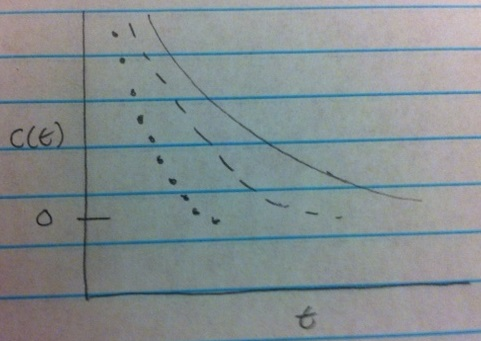
\includegraphics[scale=0.7]{4iii}
    \end{center}

    The hint provided in the problem set suggests that a denser system should take a longer period of time to become uncorrelated (reach $C(t) = 0$).

  \item This rewriting is essentially the autocorrelation function, but making use of the ``symmetry'' with regard to the number of particles, time, and dimensions. 

First, the summation makes use of the fact that particles are indistinguishable so it should not matter which specific particle we sample our autocorrelation values from. We can leverage this and instead sample the autocorrelation values for all particles at each simulation time step to get more data per step.

Secondly, the integral makes use of temporal ``symmetry'' meaining that $C(t)$ is only a function of $t$ and not of the reference state. The proof/rationalization/description for this was provided in problem set 9.

The factor of 2 accounts for the fact that our simulation takes place in 2D and that the $x$ and $y$ components of the velocity are independent of one another. Thus we can sample from both components, treating the data independently to again limit simulation time.

  \item Below is my plot for $C(t)$.
    \begin{center}
      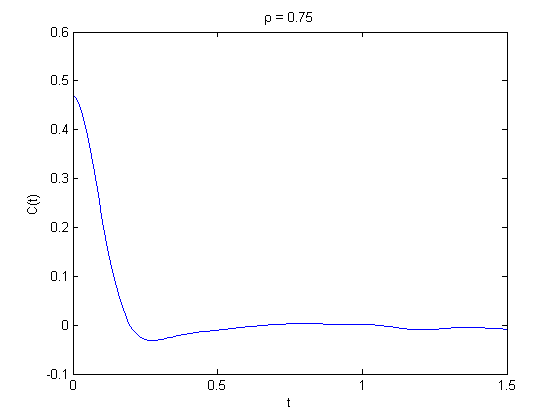
\includegraphics[scale=0.7]{4v}
    \end{center}

  \item Below is my plot for $C(t)$ at various densities.
    \begin{center}
      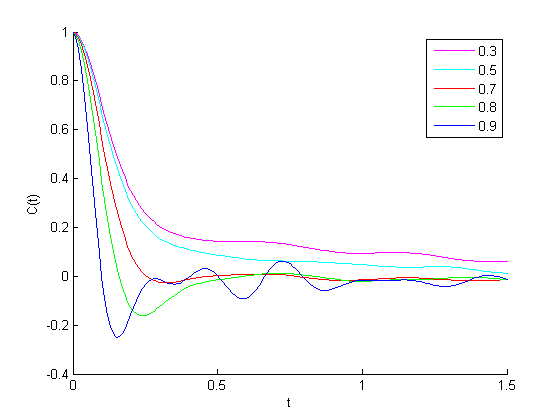
\includegraphics[scale=0.7]{4vi}
    \end{center}
    
    Contrary to my expectations (see part (iii)), from the plot above it looks like the more dense systems actually become uncorrelated faster than the less dense systems. I've double-, and triple-checked my code (see \textit{LJSimulation} and \textit{prob4.m}) and I can't find a bug. I assume there is a bug because of the hint provided in part(iii) which seems to suggest the opposite phenomenon.

    However, grasping at straws here..., my result could make sense if we consider the fact that in a dense system a particle's velocity will become uncorrelated at a faster rate because it is bouncing around so often. Whereas in a less dense system the particle is colliding less frequently with others and so it retains memory for a longer period of time. For instance, in the extreme case, consider a particle that never collides with another. Then that particle's velocity is completely correlated throughout the course of the simulation.

\end{enumerate}

\end{document}
